% Created 2025-07-09
% Intended LaTeX compiler: pdflatex
\documentclass[11pt,a4paper]{article}

% ──────────────────────── Paquetes básicos ────────────────────────
\usepackage[utf8]{inputenc}
\usepackage[T1]{fontenc}
\usepackage[english, spanish]{babel}
\usepackage{graphicx}
\usepackage{grffile}
\usepackage{longtable}
\usepackage{wrapfig}
\usepackage{rotating}
\usepackage[normalem]{ulem}
\usepackage{amsmath, amssymb}
\usepackage{textcomp}
\usepackage{capt-of}
\usepackage{tabularx}
\usepackage{lastpage}
\usepackage{enumitem}
\usepackage[table,xcdraw]{xcolor}
\usepackage[left=2.00cm,right=2.50cm,top=2.50cm,bottom=2.50cm]{geometry}
\usepackage{hyperref}

% ──────────────────────── Comandos útiles ────────────────────────
\newcommand*{\autor}[1]{\def\authorname{#1}}
\newcommand*{\titulo}[1]{\def\@title{#1}\def\ttitle{#1}}
\newcommand{\versionActual}{A}
\newcommand{\fechaA}{09/07/2025}
\newcommand{\fechaB}{}
\newcommand{\fechaC}{}
\newcommand{\docCode}{\normalsize RETRO\_GAME-DD versión \versionActual}

\titulo{Videojuego portátil inspirado en consolas retro}      % <─ Cambia si quieres
\autor{Lic. Jezabel Danon}

\usepackage{ifthen}
\newcommand{\fechaActual}{%
  \ifthenelse{\equal{\versionActual}{A}}{\fechaA}{%
    \ifthenelse{\equal{\versionActual}{B}}{\fechaB}{%
      \ifthenelse{\equal{\versionActual}{C}}{\fechaC}{
        N/A
      }}}}

% ──────────────────────── Encabezado / pie ────────────────────────
\usepackage{fancyhdr}
\fancyhf{}
\pagestyle{fancy}
\lhead{
\includegraphics[width=3.5cm]{../Figuras/logoFIUBA.pdf}}
\rhead{\normalsize\textbf{\@title}\\Documento de diseño de software\\\docCode}
\setlength{\headheight}{42pt}
\setlength{\footskip}{25pt}
\cfoot{\normalsize Página \thepage\ de \pageref{LastPage}}
\renewcommand{\headrulewidth}{1pt}
\renewcommand{\footrulewidth}{0.4pt}

% ──────────────────────── Hyperref ────────────────────────
\hypersetup{
  colorlinks=true,
  linkcolor=black,
  urlcolor=blue,
  pdftitle={\@title},
  pdfauthor={\authorname},
  pdflang={es}
}

% ──────────────────────── Documento ────────────────────────
\begin{document}

% ---------- Portada ----------
\begin{titlepage}
  \centering
  
\includegraphics[width=.7\textwidth]{../Figuras/logoFIUBA.pdf}\par
  \vspace{1cm}
  {\Huge\textbf{\ttitle}}\par
  \vspace{1.5cm}
  {\Large\itshape Documento de diseño de software (SDD)\par}
  \vspace{3cm}
  \flushleft
  {\normalsize Autor:}\par
  {\Large \authorname\ (jezabel.danon@gmail.com)}\par
  \vspace{1.5cm}
  {\scshape\LARGE \fechaActual}\par
  {\scshape\LARGE Versión \versionActual}\par
  \vfill
  \centering
  \textit{Basado en el estándar IEEE 1016-2017.}
\end{titlepage}

\clearpage            % fuerza una nueva página real
\pagestyle{fancy}     % activa encabezado y pie desde esta página

\section*{Historial de cambios}
\pagestyle{fancy}     % activa el estilo fancy para el resto
\begin{table}[ht]
\label{tab:registro}
\centering
\begin{tabularx}{\linewidth}{@{}|c|c|X|c|c|@{}}
\hline
\rowcolor[HTML]{C0C0C0} 
Versión & Fecha & \multicolumn{1}{c|}{\cellcolor[HTML]{C0C0C0}Descripción}  & Autor & Revisores     \\ \hline
A   & \fechaA   & Creación del documento     & \authorname     &                        \\ \hline
\end{tabularx}
\end{table}

\pagebreak

\clearpage
\tableofcontents
\clearpage

% ---------- 1 Introducción ----------
\section{Introducción}
\subsection{Propósito}
\begin{enumerate}
  \item Este documento describe el diseño del software para el sistema embebido \textit{\ttitle}. 
  \item Está dirigido a los desarrolladores que se ocupen del análisis, diseño e implementación del software, así como también a quienes desarrollen el testing, validaciones y/o verificaciones del mismo.
\end{enumerate}

\subsection{Ámbito}
\begin{enumerate}
  \item El sistema está compuesto por un dispositivo embebido portátil que integra entradas físicas (botones, joystick, acelerómetro), salidas audiovisuales (pantalla, parlante, vibración) y una unidad de procesamiento encargada de coordinar la ejecución de un demo de juego simple.
  \item El presente diseño de software abarca los módulos encargados de:
  \begin{itemize}
    \item Control de entrada/salida digital y analógica.
    \item Gestión del flujo del juego.
    \item Renderizado gráfico en pantalla.
    \item Generación de audio y control de vibración.
    \item Manejo de estados internos y lógica de juego.
  \end{itemize}
  \item Este documento se enfoca exclusivamente en la descripción estructural y funcional del software embebido. No se incluyen aspectos de diseño físico, elección final de componentes electrónicos ni pruebas de verificación, los cuales son abordados en documentos específicos (como las especificaciones de hardware o el plan de validación).
  \item El diseño cubre las capas de abstracción de hardware (drivers), lógica de control del juego, gestión de recursos gráficos y sonoros, así como el manejo de entradas y salidas del sistema. 
  \item Quedan fuera de este documento los detalles de bajo nivel sobre protocolos específicos de comunicación (como I\textsuperscript{2}C o SPI), que se encuentran documentados en los manuales de componentes o en la especificación de hardware.
  \item Tampoco se incluyen aspectos de programación de la interfaz de usuario en cuanto a estilo o experiencia visual final, los cuales podrán ser definidos en una etapa posterior del desarrollo.
\end{enumerate}

\subsection{Definiciones y acrónimos}
  \begin{enumerate}
    \item IEEE: Instituto de Ingenieros Eléctricos y Electrónicos.
    \item ERS: Especificación de Requisitos de Software.
    \item RTOS: Sistema Operativo de Tiempo Real (Real Time Operating System).
    \item CMSIS: Arm's Common Microcontroller Software Interface Standard. Se compone por un conjunto de APIS, componentes de software, herramientas y flujos de trabajo provisto por el desarrollador de la arquitectura del microcontrolador a utilizar.
    \item HAL: Hardware Abstraction Layer. Conjunto de bibliotecas de software provistas por STMicroelectronics para simplificar la interacción con el hardware de microcontroladores STM32.
    \item UI: Interfaz de usuario (User Interface).
    \item UART: Universal Asynchronous Receiver/Transmitter. 
    \item I2C: Inter-Integrated Circuit.
    \item SPI: Serial Peripheral Interface.
    \item ADC: Analogic to Digital Converter.
    \item PWM: Pulse Width Modulation.
    \item GPIO: General-purpose Input/Output.
    \item ST-Link: programador y depurador integrado en placas STM32.
    \item N/A: No Aplica.
  \end{enumerate}

\subsection{Referencias}

\begin{enumerate}
  \item Estándar IEEE 1016-2017.
  \item \href{https://drive.google.com/file/d/1C3vEYR8wME6EzlZVVC-gT2u86dwnoZA-/view?usp=sharing}{Plan de proyecto del trabajo práctico final} para la \textit{Carrera de Especialización en Sistemas Embebidos} (RETRO\_GAME-PP-v5). 
  \item Especificaciones de requisitos de hardware: RETRO\_GAME-RH-vA.
  \item Especificaciones de requisitos de software: RETRO\_GAME-RS-vA.
\end{enumerate}

% ---------- 2 Visión general de la arquitectura ----------
\section{Visión general de la arquitectura}

\subsection{Perspectiva y motivación}
\begin{enumerate}
  \item Esta sección describe la estructura general del sistema \textit{\ttitle} desde una perspectiva arquitectónica. 
  \item Se presenta una vista de alto nivel que permite comprender los principales módulos de software, su organización y las interacciones entre ellos.
  \item La arquitectura fue diseñada con el objetivo de facilitar el desacoplamiento entre módulos funcionales y la posibilidad de incorporar nuevas funcionalidades con un impacto mínimo en el resto del sistema.
\end{enumerate}

\subsection{Contexto del sistema}
\begin{enumerate}
  \item El software embebido diseñado es autónomo, no interactúa con sistemas externos ni depende de servicios de red.
  \item La única interfaz externa habilitada será mediante UART vía ST-Link, utilizada para depuración durante el desarrollo.
\end{enumerate}

\subsection{Vista en capas}
\begin{enumerate}
  \item El sistema está estructurado en tres secciones o capas principales, siguiendo un enfoque jerárquico:
  \begin{itemize}
    \item \textbf{Capa de Drivers:} contiene los controladores de hardware y sus rutinas de inicialización. Se encarga del acceso a periféricos como pantalla, audio, EEPROM, entradas físicas, temporizadores y comunicación serie.
    \item \textbf{Capa de lógica del sistema:} incluye los módulos que gestionan el estado global del sistema, la persistencia, los menús de usuario, la carga de recursos y la gestión de entradas. Esta capa implementa las FSMs de alto nivel del sistema y coordina el flujo entre modos.
    \item \textbf{Capa de lógica del juego:} implementa la lógica específica de gameplay, el renderizado de escenas y la interpretación de las entradas como acciones del juego.
  \end{itemize}
  \item Esta separación facilita la mantenibilidad y escalabilidad del sistema. La Figura~\ref{fig:diagCapas} ilustra esta organización.
  \item Cabe destacar que en la Figura~\ref{fig:diagCapas} también se incluyen capas provistas por la plataforma, como CMSIS, HAL y RTOS. Estas capas no forman parte del diseño detallado presentado en este documento, pero se incluyen para brindar una visión completa del entorno sobre el cual se construye el software.
\end{enumerate}

\begin{figure}[h]
\centering 
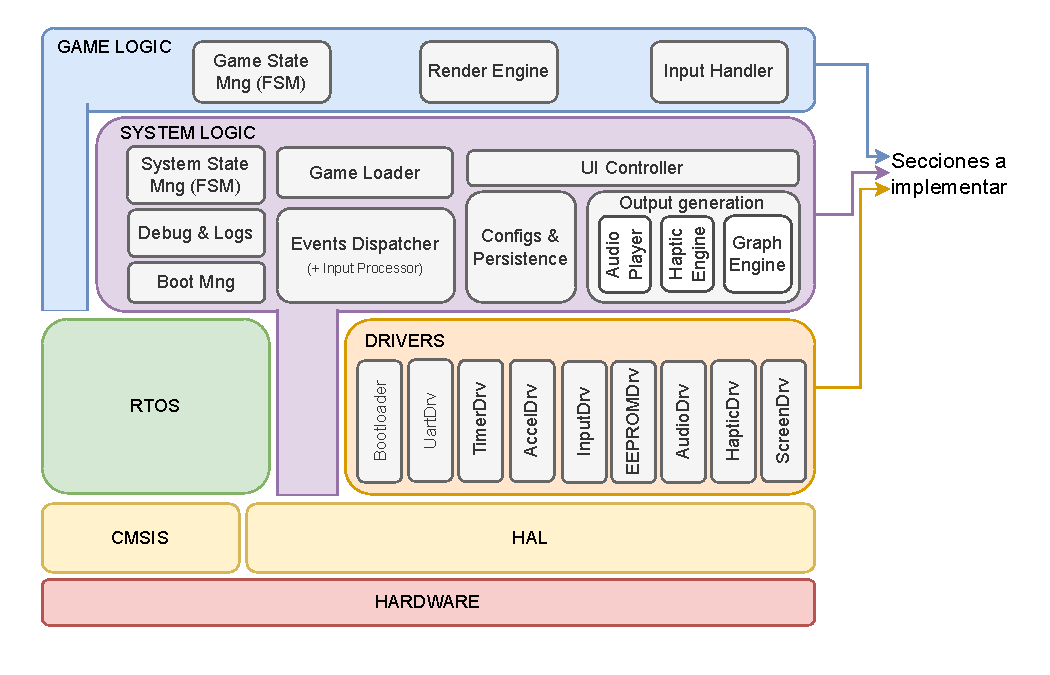
\includegraphics[width=.85\textwidth]{../Figuras/SW_layers.pdf}
\caption{Diagrama de capas del sistema.}
\label{fig:diagCapas}
\end{figure}

\subsection{Estilos y patrones arquitectónicos}
\begin{enumerate}
  \item \textbf{Estilo por capas:} el sistema seguirá una arquitectura en capas, separando claramente la interacción con el hardware, la lógica de sistema y la lógica de juego. Esto permite modularidad, testeabilidad y mantenimiento desacoplado.
  \item \textbf{Patrón de máquina de estados finitos (FSM):} tanto el flujo del sistema (menú, splash, juego, pausa) como el gameplay utilizarán FSMs explícitas para representar y gestionar los modos de operación y transición entre ellos.
  \item \textbf{RTOS cooperativo:} el sistema se ejecutará sobre un RTOS (pen particular será FreeRTOS), con tareas cooperativas y temporizadas. Se definirán prioridades fijas para cada servicio.
  \item \textbf{Modelo combinado productor-consumidor / publicación-suscripción:} 
  \begin{itemize}
    \item En los casos donde un módulo conoce explícitamente a su receptor, se adoptará un esquema de productor-consumidor (1:1). 
    \item En cambio, para eventos globales que deben ser observados por múltiples componentes, se utilizará el patrón de publicación/suscripción (1:N). 
  \end{itemize}
  \item \textbf{Separación lógica-física:} los servicios que gestionan el estado del juego y las interfaces de usuario están desacoplados de los drivers físicos, permitiendo una posible reutilización o simulación.
\end{enumerate}

% ---------- 3 Descripción de módulos y servicios ----------
\section{Descripción de módulos y servicios}

%%%%%%%%%%%%%%%%%%%%%%%%%%%%%%%%%%%%%%%%%%%%%%%%%%%%%%%%%%%%
% 3.1 DRIVERS                                      %
%%%%%%%%%%%%%%%%%%%%%%%%%%%%%%%%%%%%%%%%%%%%%%%%%%%%%%%%%%%%
\subsection{Boot y drivers}

%----------------------------------------------------------
\subsubsection{AccelDrv}
\begin{itemize}
  \item \textbf{Identificador:} AccelDrv
  \item \textbf{Responsabilidad principal:} Lectura de acelerómetro por I\textsuperscript{2}C; genera IRQ “data ready”.
  \item \textbf{Interfaces}
    \begin{itemize}
      \item API: \texttt{AccelDrv\_Init()}, \texttt{AccelDrv\_Read(float* xyz)}.
      \item Evento publicado: \texttt{ACCEL\_DATA\_READY(x,y,z)} a la cola de alto nivel.
    \end{itemize}
  \item \textbf{Datos utilizados:} Buffer \texttt{int16\_t raw[3]}, escala de sensado.
  \item \textbf{Dependencias:} I\textsuperscript{2}C HAL, TimerDrv (timeouts).
  \item \textbf{Errores y manejo:} NACK o timeoutm → evento \texttt{ACCEL\_ERR}.
  \item \textbf{Notas especiales:} Tasa de muestreo fija a 100 Hz (configurable).
\end{itemize}

%----------------------------------------------------------
\subsubsection{EEPROMDrv}
\begin{itemize}
  \item \textbf{Identificador:} EEPROMDrv
  \item \textbf{Responsabilidad principal:} Lectura/escritura de páginas vía I\textsuperscript{2}C; verificación de ACK y CRC.
  \item \textbf{Interfaces}
    \begin{itemize}
      \item API síncrona: \texttt{EEPROMDrv\_ReadPage(addr,\*buf)}, \texttt{EEPROMDrv\_WritePage(addr,\*buf)}.
      \item Evento asíncrono: \texttt{EEPROM\_DONE} / \texttt{EEPROM\_ERR}.
    \end{itemize}
  \item \textbf{Datos utilizados:} Buffer página 64 B, mapa de snapshots, checksum.
  \item \textbf{Dependencias:} I\textsuperscript{2}C HAL.
  \item \textbf{Errores y manejo:} Reintenta 3 veces; si persiste → evento \texttt{EEPROM\_ERR}.
  \item \textbf{Notas:} Opera en modo DMA para transferencias largas.
\end{itemize}

%----------------------------------------------------------
\subsubsection{ScreenDrv}
\begin{itemize}
  \item \textbf{Identificador:} ScreenDrv
  \item \textbf{Responsabilidad principal:} Inicializa el controlador ST7735, gestiona ventana y transferencias DMA-SPI de píxeles (doble buffer).
  \item \textbf{Interfaces}
    \begin{itemize}
      \item API: \texttt{ScreenDrv\_Init()}, \texttt{ScreenDrv\_SwapBuffers()}.
      \item Evento \texttt{FRAME\_DONE} al terminar DMA.
    \end{itemize}
  \item \textbf{Datos utilizados:} Dos frame-buffers de 160×128×16 bpp.
  \item \textbf{Dependencias:} SPI HAL, DMA2, TimerDrv (VSync simulado).
  \item \textbf{Errores y manejo:} Timeout SPI, re-init de controlador.
\end{itemize}

%----------------------------------------------------------
\subsubsection{AudioDrv}
\begin{itemize}
  \item \textbf{Identificador:} AudioDrv
  \item \textbf{Responsabilidad principal:} Reproduce audio mediante PWM + DMA circular; controla volumen analógico (pin GPIO).
  \item \textbf{Interfaces} 
    \begin{itemize}
      \item API: \texttt{AudioDrv\_Play(buf,len)}, \texttt{AudioDrv\_SetVolume(uint8)}.
      \item Evento \texttt{AUDIO\_UNDERRUN} si el búfer se vacía.
    \end{itemize}
  \item \textbf{Datos utilizados:} Búfer de 1024 muestras 8 bit.
  \item \textbf{Dependencias:} TIM PWM, DMA Stream 1.
  \item \textbf{Errores y manejo:} Underrun → rellena con silencio.
\end{itemize}

%----------------------------------------------------------
\subsubsection{HapticDrv}
\begin{itemize}
  \item \textbf{Identificador:} HapticDrv
  \item \textbf{Responsabilidad principal:} Dispara patrones en el DRV2605L mediante I\textsuperscript{2}C.
  \item \textbf{Interfaces} 
    \begin{itemize}
      \item API: \texttt{HapticDrv\_PlayPattern(uint8 id)}.
      \item Notificación \texttt{HAPTIC\_DONE} cuando finaliza el patrón.
    \end{itemize}
  \item \textbf{Datos utilizados:} Cola circular de 8 patrones.
  \item \textbf{Dependencias:} I\textsuperscript{2}C HAL.
  \item \textbf{Errores y manejo:} Si no hay ACK → descarta patrón y genera \texttt{HAPTIC\_ERR}.
\end{itemize}

%----------------------------------------------------------
\subsubsection{UARTDrv}
\begin{itemize}
  \item \textbf{Identificador:} UARTDrv
  \item \textbf{Responsabilidad principal:} Comunicación serie (USART2) con DMA; expone \texttt{UartDrv\_Write()} y \texttt{UartDrv\_Read()}.
  \item \textbf{Dependencias:} DMA Stream 6/7, HAL UART.
  \item \textbf{Errores y manejo:} Overflow RX → descarta byte y cuenta error.
\end{itemize}

\subsubsection{InputDrv}
\begin{itemize}
  \item \textbf{Identificador:} InputDrv
  \item \textbf{Responsabilidad principal:} Unifica lectura de botones (GPIO + EXTI) y joystick (ADC DMA continuo), aplica antirrebote y dead-zone.
  \item \textbf{Interfaces}
    \begin{itemize}
      \item \texttt{InputDrv\_RegisterCallback(cb)}.
      \item Evento \texttt{INPUT\_RAW(btnMask, joyX, joyY)} cada 10 ms.
    \end{itemize}
  \item \textbf{Dependencias:} HAL GPIO, ADC DMA.
\end{itemize}

\subsubsection{TimerDrv}
\begin{itemize}
  \item \textbf{Identificador:} TimerDrv
  \item \textbf{Responsabilidad principal:} Genera interrupción \texttt{FRAME\_TICK} cada 50 ms (20 FPS) y timers de usuario.
  \item \textbf{Interfaces:} \texttt{TimerDrv\_Start(freq)}, callback global.
  \item \textbf{Dependencias:} TIM3.
\end{itemize}

%%%%%%%%%%%%%%%%%%%%%%%%%%%%%%%%%%%%%%%%%%%%%%%%%%%%%%%%%%%%
% 3.2 LÓGICA DEL SISTEMA                                   %
%%%%%%%%%%%%%%%%%%%%%%%%%%%%%%%%%%%%%%%%%%%%%%%%%%%%%%%%%%%%
\subsection{Lógica del sistema}

\subsubsection{Boot Manager}
\begin{itemize}
  \item \textbf{Identificador:} BootMgr
  \item \textbf{Responsabilidad principal:} Inicializa RTOS, crea colas, verifica drivers, muestra logo y transfiere a \texttt{SYS\_MAIN\_MENU}.
  \item \textbf{Interfaces}
    \begin{itemize}
      \item Entradas: eventos \texttt{DRIVER\_OK[i]}
      \item Salidas: \texttt{ENTER\_SPLASH}, \texttt{GO\_MENU}
    \end{itemize}
  \item \textbf{Dependencias:} Todos los drivers.
\end{itemize}

\subsubsection{Resource Loader}
\begin{itemize}
  \item \textbf{Identificador:} ResLoader
  \item \textbf{Responsabilidad principal:} Carga assets (sprites, fuentes, jingles) en RAM desde EEPROM o Flash.
  \item \textbf{Interfaces} 
    \begin{itemize}
      \item \texttt{ResLoader\_Request(type,id)}, callback \texttt{RES\_READY(ptr)}.
    \end{itemize}
  \item \textbf{Dependencias:} EEPROMDrv, Graphics Engine, Audio Player.
  \item \textbf{Notas:} Sólo lectura; nunca escribe EEPROM.
\end{itemize}

\subsubsection{Config \& Persistence}
\begin{itemize}
  \item \textbf{Identificador:} ConfigPersist
  \item \textbf{Responsabilidad principal:} Guarda / carga snapshot de juego y ajustes; publica \texttt{HAS\_SAVE}, \texttt{SAVE\_OK}, \texttt{SAVE\_ERR}.
  \item \textbf{Interfaces} 
    \begin{itemize}
      \item API síncrona: \texttt{Persist\_Save(ptr,len)}, \texttt{Persist\_Load(ptr,len)}.
      \item Eventos: véase arriba.
    \end{itemize}
  \item \textbf{Dependencias:} EEPROMDrv, CRC util.
\end{itemize}

\subsubsection{Event Dispatcher}
\begin{itemize}
  \item \textbf{Identificador:} EventDisp
  \item \textbf{Responsabilidad principal:} Recibe eventos de bajo nivel (inputs, ticks), los normaliza y redistribuye a colas de alto nivel.
  \item \textbf{Notas:} Punto único de entrada al sistema lógico.
\end{itemize}

\subsubsection{UI Controller}
\begin{itemize}
  \item \textbf{Identificador:} UIController
  \item \textbf{Responsabilidad principal:} Maneja menús (Splash, Main Menu, Pausa), dibuja con Graphics Engine y envía acciones (\texttt{NEW\_GAME}, \texttt{LOAD\_SAVE}).
  \item \textbf{Dependencias:} Graphics Engine, Audio Player, Haptic Engine.
\end{itemize}

\subsubsection{Graphics Engine}
\begin{itemize}
  \item \textbf{Identificador:} GfxEng
  \item \textbf{Responsabilidad principal:} Primitivas 2-D, doble buffer, envía display-list a ScreenDrv.
\end{itemize}

\subsubsection{Audio Player}
\begin{itemize}
  \item \textbf{Identificador:} AudPlayer
  \item \textbf{Responsabilidad principal:} Mezcla música y SFX, gestiona mute global.
\end{itemize}

\subsubsection{Haptic Engine}
\begin{itemize}
  \item \textbf{Identificador:} HapEng
  \item \textbf{Responsabilidad principal:} Cola de patrones y temporización para DRV2605L.
\end{itemize}

\subsubsection{Debug \& Logs}
\begin{itemize}
  \item \textbf{Identificador:} LogSink
  \item \textbf{Responsabilidad principal:} Enrutamiento de \texttt{Log\_Put()} a UART, comandos \texttt{logon}/\texttt{logoff}.
\end{itemize}

\subsubsection{System State Mng}
\begin{itemize}
  \item \textbf{Identificador:} SysState
  \item \textbf{Responsabilidad principal:} FSM del sistema (\texttt{SYS\_SPLASH}, \texttt{SYS\_MENU}, \texttt{SYS\_IN\_GAME}, \texttt{SYS\_PAUSED}).
\end{itemize}

\subsubsection{Game Loader}
\begin{itemize}
  \item \textbf{Identificador:} GameLoader
  \item \textbf{Responsabilidad principal:} Decide nueva partida vs. snapshot, solicita assets y variables iniciales.
\end{itemize}

%%%%%%%%%%%%%%%%%%%%%%%%%%%%%%%%%%%%%%%%%%%%%%%%%%%%%%%%%%%%
% 3.3 LÓGICA DEL JUEGO                                     %
%%%%%%%%%%%%%%%%%%%%%%%%%%%%%%%%%%%%%%%%%%%%%%%%%%%%%%%%%%%%
\subsection{Lógica del juego}

\subsubsection{Game State Mng}
\begin{itemize}
  \item \textbf{Identificador:} GameState
  \item \textbf{Responsabilidad principal:} Ejecuta bucle de juego; pasa a \texttt{GAME\_FROZEN} al pausar, procesa \texttt{RESUME} o \texttt{EXIT}.
\end{itemize}

\subsubsection{Render Engine (Juego)}
\begin{itemize}
  \item \textbf{Identificador:} GameRender
  \item \textbf{Responsabilidad principal:} Construye display-list cada frame y la envía a GfxEng.
\end{itemize}

\subsubsection{Input Handler (Juego)}
\begin{itemize}
  \item \textbf{Identificador:} GameInput
  \item \textbf{Responsabilidad principal:} Traduce eventos normalizados a acciones de gameplay (mover, disparar, etc.).
\end{itemize}

% ---------- 4 Modelos dinámicos ----------
\section{Modelos dinámicos}
\subsection{Diagrama de secuencia 1 - Encendido hasta menú}
% \begin{center}
% %   \includegraphics[width=.9\linewidth]{Figuras/seq_boot_to_menu.pdf}
% \end{center}
Descripción narrativa de cada paso.

\subsection{Diagrama de secuencia 2 - Pausa y opciones}
% \begin{center}
%   \includegraphics[width=.9\linewidth]{Figuras/seq_pause_menu.pdf}
% \end{center}

% ---------- 5 Asignación a tareas y concurrencia ----------
\section{Concurrencia y asignación a tareas}
\subsection{Mapa de tareas FreeRTOS}
Tabla con tareas, prioridad, stack, frecuencia.

\subsection{Sincronización y comunicación}
Colas, semáforos, exclusiones mutuas usadas.

% ---------- 6 Aspectos de datos ----------
\section{Modelo de datos}
\subsection{Estructuras persistentes}
Formato del snapshot de partida, layout EEPROM, checksum.

\subsection{Estructuras en RAM}
Buffers de audio, frame buffer, colas de eventos.

% ---------- 7 Manejo de errores y registro (logging) ----------
\section{Manejo de errores y logging}
Política de códigos de error, niveles de log, rutas de fallos críticos.

% ---------- 8 Requisitos de diseño no funcionales ----------
\section{Requisitos de diseño no funcionales}
Rendimiento (FPS), footprint de Flash/RAM, respuesta a interrupciones, requisitos de seguridad.

% ---------- 9 Referencias ----------
\section{Referencias}
\bibliographystyle{plain}
% \bibliography{biblio_design}

% ---------- Apéndices ----------
\appendix
\section{Apéndice A - Glosario completo de servicios}
Tabla resumen: Nombre, capa, descripción de 1 línea.

\section{Apéndice B - Diagramas adicionales}
Coloca aquí otros diagramas UML o listas de mensajes.

\end{document}
